\chapter{Senzory}
\label{sec:Sensors}
\vspace{-20pt}
\

Platforma FRDM-K66F obsahuje tří senzory, které tvoří
9-osou IMU jednotku. Konkretně jako akcelerometr a magnetometr deska má
NXP FXOS8700CQ a gyroskop NXP FXAS21002. Tyto senzory komunikují s platformou
pomocí $I^2C$\cite{frdmk66UserGuide}.

\section{NXP FXOS8700CQ}\

\textbf{NXP FXOS8700CQ} je pokročilý 6-osy senzor,
který kombinuje funkce 3-os akcelerometru
a 3-os magnetometru do jednoho čipu. Akcelerometr v senzoru FXOS8700CQ má
nastavitelné rozsahy ±2 g, ±4 g, ±8 g s 14-bitovým rozlišením, zatímco magnetometr
poskytuje 16-bitové rozlišení s rozsahem ±1200 µT na osu. Pro komunikaci podporuje
$I^2C$ a SPI rozhraní. Má dva piny pro~přerušení a podporuje odesílat data rychlosti
až 800 Hz pro každý senzor a až 400 Hz v hybridním režimu.
Tato~integrace umožňuje zařízení zachytit komplexní data o svém pohybu a
orientaci vůči zemskému gravitačnímu a magnetickému poli.
Orientace akcelerometru a magnetometru je na obrázku \ref{fig:FXOS_Orientation}
\cite{FXOS8700CQ}.

\begin{figure}[!h]
    \centering
    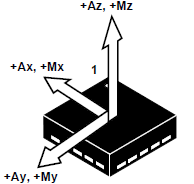
\includegraphics[width = 0.5\linewidth]{Figures/FXOS_Orientation.png}
    \caption{NXP FXOS8700CQ orientace\cite{FXOS8700CQ}.}
    \label{fig:FXOS_Orientation}
\end{figure}

\section{NXP FXAS21002}\

\textbf{NXP FXAS21002} je vysoce výkonný 3-osy senzor, který poskytuje data o úhlové rychlosti
zrychlení. Tento senzor má nastavitelné rozsahy ±250, ±500, ±1000, a
±2000 stupňů za sekundu
s 16-bitovým rozlišením. Pro komunikaci podporuje $I^2C$ a SPI rozhraní.
Má dva piny pro přerušení a podporuje odesílat data rychlosti až 800 Hz.
To umožňuje zařízení detekovat rotace kolem svych os.
Orientace gyroskopu je na obrázku \ref{fig:FXAS_Orientation}\cite{FXAS21002}.

\begin{figure}[!h]
    \centering
    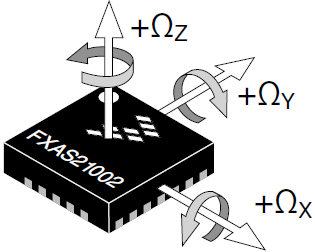
\includegraphics[width = 0.5\linewidth]{Figures/FXAS_Orientation.png}
    \caption{NXP FXAS21002 orientace\cite{FXAS21002}.}
    \label{fig:FXAS_Orientation}
\end{figure}

\endinput
